\section{Appendices}
\subsection{Code}
The python code with documentation is available on GitHub at:\\ \url{https://github.com/clucas111/delineating-linear-elements}

\subsection{Data}
The data is available at:\\
\url{https://drive.google.com/open?id=0BwxnnB9jCFE5Q2dVRlRxUHBlV1E}

\subsection{GIS}
The maps, rasters, and features are available on GitHub at:\\
\url{https://github.com/clucas111/delineating-linear-elements}

\subsection{Ground survey}
The photos are available at:\\
\url{https://drive.google.com/open?id=0BwxnnB9jCFE5cmJIUm1hbzhrb0k}
\\
The approximate locations of the photos are shown in figure \ref{fig:photolocs}. A more detailed map is available in the folder on Google Drive.

\begin{figure}
	\centering
	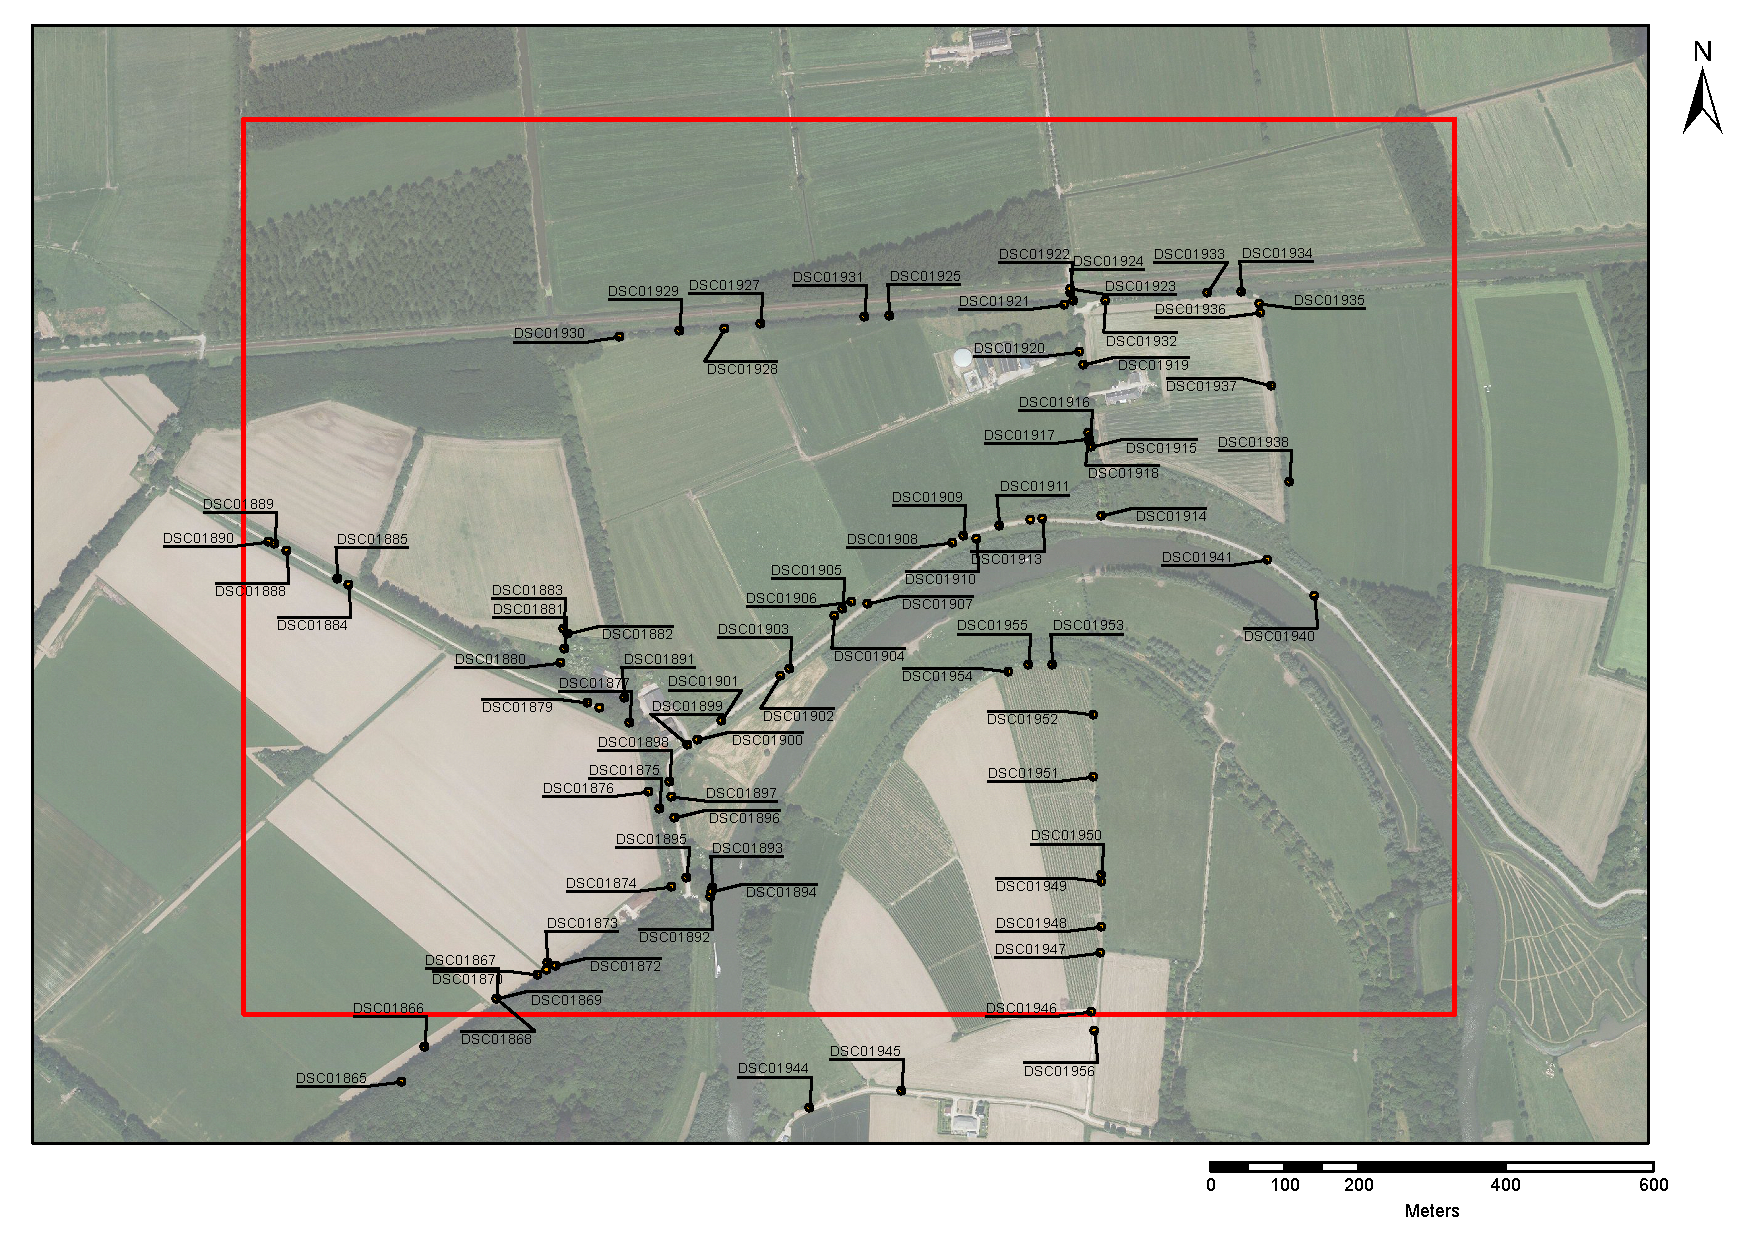
\includegraphics[scale=0.45]{./img/PhotoLocations}
	\caption{The approximate locations of the photos.}
	\label{fig:photolocs}
\end{figure}

\pagebreak
\subsection{Detailed Work Flow}
\subsubsection{Data preprocessing}
	\begin{itemize}
		\item Download LAZ data from PDOK
		\item Extract study area to LAS using laszip (LASTools)
		\item Spatially downsample to 0.3m distance between all points using CloudCompare (reduces effects of overlapping scans on computation of features)
		\item Convert LAS to CSV using las2txt (LASTools)
		\item Read CSV into python using pandas
	\end{itemize}

\subsubsection{Feature extraction}
	\begin{itemize}
		\item Compute nearest neighbours using a k-d tree
		\item Compute basic geometric properties and structure tensors of neighbourhoods
		\item Compute structure tensor features
		\item Remove irrelevent points based on sphericity and planarity
		\item Compute normalized return number
		\item Write point features to CSV
	\end{itemize}

\subsubsection{Classification}
	\begin{itemize}
		\item Data preparation
		\begin{itemize}
			\item Manually segment areas of the two classes in the point cloud using CloudCompare's segment tool
			\item Save the two segmented point clouds as CSV
			\item Read the two CSV files into python as dataframes using pandas
			\item Merge the two dataframes, adding a column indicating the class
			\item Define the feature space to use during classification
			\item Drop highly correlated features from the feature space by computing pearson correlation coefficient between all features.
		\end{itemize}

		\item Parameter optimization (Grid Search)
		\begin{itemize}
			\item Define a parameter grid to search in
			\item Split the data into 3 folds
			\item Loop through each fold and through each combination in the parameter grid
			\begin{itemize}
				\item Create a balanced random forest classifier
				\item Fit the training data to classifier
				\item Assess the performance of classifier using the accuracy metrics
			\end{itemize}
			\item Choose the best parameters
		\end{itemize}
	
		\item Validate classifier (Cross validation)
		\begin{itemize}
			\item Split the data into 10 folds
			\item Loop through each fold
			\begin{itemize}
				\item Create a balanced random forest classifier with optimized parameters
				\item Fit the training data to classifier
				\item Assess the performance of classifier using the accuracy metrics
			\end{itemize}
		\end{itemize}
	
		\item Classify vegetation
		\begin{itemize}
			\item Load CSV of the entire point cloud with computed features
			\item Create a balanced random forest classifier with optimized parameters
			\item Fit classifier with manually segmented data
			\item Predict classes of the unknown points
		\end{itemize}
	
		\item Classify trees \& vegetation
		\begin{itemize}
			\item Compute cylindrical neighbourhoods using a k-d tree
			\item Classify into trees \& vegetation based on height difference
		\end{itemize}
	
		\item Write x, y, z coordinates and class of points to CSV
	\end{itemize}

\subsubsection{Delineate linear elements}
	\begin{itemize}
		\item Data preparation
		\begin{itemize}
			\item Load CSV with the points and their classes
			\item Write CSV with just x and y coordinates for each class
			\item Downsample point cloud using the CSVs and CloudCompare
			\item Load resulting CSVs into python
			\item Shift coordinates to 0, 0
		\end{itemize}
		
		\item Delineate linear elements - Manual
		\begin{itemize}
			\item Create polygon from all points from each class
			\item Export polygons to shapefiles
			\item Load shapefiles in ArcGIS
			\item Single to multi polygon (ArcGIS tool)
			\item Manually delineate linear elements in resulting polygons
		\end{itemize}
		
		\item Delineate linear elements - Automated
		\begin{itemize}
			\item Segment rectangular regions
			\begin{itemize}
				\item While there are points left:
				\begin{itemize}
					\item Initiate starting region (point with minimal x and its 19 closest neighbours)
					\item Add points as long as region stays above rectangularity threshold
				\end{itemize}
			\end{itemize}
		
			\item Convert regions to polygons
			\item Merge objects if they are in proximity, in the same direction and aligned with each other
			\item Export polygons to shapefile
		\end{itemize}
		
		\item Assess accuracy
		\begin{itemize}
			\item Load automated and manual shapefiles in ArcGIS
			\item Create difference features (TP, TN, FP, FN) using the intersect \& difference tools
			\item Check the areas using the statistics of the \textit{Shape\_Area} field
			\item Create confusion matrices
			\item Calculate corresponding accuracy metrics
		\end{itemize}
	\end{itemize}

\subsection{Detailed Overview of Software}
\footnotesize
\renewcommand{\labelitemi}{$\cdot$}
\begin{longtable}{ p{0.2\textwidth} p{0.4\textwidth} p{0.3\textwidth} }
	\caption{An overview of all the software used, and what it was utilized for.}
	\label{tab:software}
	\\
	\toprule
	Software & Official Description & Our Application\\
	\midrule
	\endhead
	
	\addlinespace
	\midrule
	\multicolumn{3}{c}{Table continues on the next page..} \\
	\midrule
	\endfoot
	
	\bottomrule
	\endlastfoot
	
	LASTools & A collection of highly efficient, batch-scriptable, multicore command line tools. Tools to classify, tile, convert, filter, raster, triangulate, contour, clip, and polygonize LiDAR data. & 
	\begin{minipage}[t]{0.3\textwidth}
		\begin{itemize}[leftmargin=*,noitemsep]
			\item Decompressing LAZ to LAS
			\item Cropping data to study area
			\item Converting LAS to CSV
		\end{itemize}
	\end{minipage}\\

	\addlinespace
	CloudCompare & CloudCompare is a 3D point cloud (and triangular mesh) processing software. &
	\begin{minipage}[t]{0.3\textwidth}
	\begin{itemize}[leftmargin=*,noitemsep]
		\item Visualizing point clouds
		\item Downsampling point clouds
	\end{itemize}
	\end{minipage}\\

	\addlinespace
	ArcGIS & Use ArcMap, ArcCatalog, ArcGlobe, or ArcScene, to create maps, perform spatial analysis, manage geographic data, and share your results. &
	\begin{minipage}[t]{0.3\textwidth}
		\begin{itemize}[leftmargin=*,noitemsep]
			\item Create maps
			\item Manually delineate linear elements
			\item Analyse accuracy of delineation of linear elements (create difference map, assess area TP/TN/FP/FN)
		\end{itemize}
	\end{minipage}\\

	\addlinespace	
	Python & & 
	\begin{minipage}[t]{0.3\textwidth}
		\begin{itemize}[leftmargin=*,noitemsep]
			\item Programming language
		\end{itemize}
	\end{minipage}\\

	\addlinespace
	\ \ Spyder & Spyder is a Python development environment with a lot of features. &
	\begin{minipage}[t]{0.3\textwidth}
		\begin{itemize}[leftmargin=*,noitemsep]
			\item Integrated Development Environment (IDE)
		\end{itemize}
	\end{minipage}\\

	\addlinespace
	\ \ NumPy & NumPy is the fundamental package for scientific computing with Python. &
	\begin{minipage}[t]{0.3\textwidth}
		\begin{itemize}[leftmargin=*,noitemsep]
			\item Array objects
			\item Linear algebra (matrix operations, eigenvalues \& eigenvectors)
			\item Covariance matrix
		\end{itemize}
	\end{minipage}\\

	\addlinespace
	\ \ SciPy & SciPy library provides many user-friendly and efficient numerical routines such as routines for numerical integration and optimization. &
	\begin{minipage}[t]{0.3\textwidth}
		\begin{itemize}[leftmargin=*,noitemsep]
			\item Constructing and querying k-d trees
		\end{itemize}
	\end{minipage}\\

	\addlinespace
	\ \ pandas & pandas is an open source, BSD-licensed library providing high-performance, easy-to-use data structures and data analysis tools for the Python programming language. &
	\begin{minipage}[t]{0.3\textwidth}
		\begin{itemize}[leftmargin=*,noitemsep]
			\item DataFrame objects
			\item Read \& write CSV files
			\item Creating confusion matrices
		\end{itemize}
	\end{minipage}\\

	\addlinespace
	\ \ sklearn & scikit-learn, Machine Learning in Python &
	\begin{minipage}[t]{0.3\textwidth}
		\begin{itemize}[leftmargin=*,noitemsep]
			\item Decision tree classifiers
			\item Creating cross validation folds
			\item Creating parameter grids for optimization
			\item Accuracy metrics (ROC-AUC, MCC)
		\end{itemize}
	\end{minipage}\\

	\addlinespace
	\ \ imblearn & imbalanced-learn is a python package offering a number of re-sampling techniques commonly used in datasets showing strong between-class imbalance. &
	\begin{minipage}[t]{0.3\textwidth}
		\begin{itemize}[leftmargin=*,noitemsep]
			\item Accuracy metrics for imbalanced datasets (Geometric mean)
		\end{itemize}
	\end{minipage}\\

	\addlinespace
	\ \ matplotlib & Matplotlib is a Python 2D plotting library which produces publication quality figures in a variety of hardcopy formats and interactive environments across platforms. &
	\begin{minipage}[t]{0.3\textwidth}
		\begin{itemize}[leftmargin=*,noitemsep]
			\item Creating plots and charts
		\end{itemize}
	\end{minipage}\\

	\addlinespace
	\ \ shapely & Shapely is a BSD-licensed Python package for manipulation and analysis of planar geometric objects. &
	\begin{minipage}[t]{0.3\textwidth}
		\begin{itemize}[leftmargin=*,noitemsep]
			\item Polygon geometry object
			\item Converting triangles to polygon
		\end{itemize}
	\end{minipage}\\

	\addlinespace
	\ \ fiona & Fiona is OGR's neat and nimble API for Python programmers. &
	\begin{minipage}[t]{0.3\textwidth}
		\begin{itemize}[leftmargin=*,noitemsep]
			\item Export polygons to shapefile
		\end{itemize}
	\end{minipage}\\

\end{longtable}

\subsection{Exercise Point Cloud Classification}
An assignment to introduce classifying a point cloud in python was made to facilitate a continuation of this research by other researchers. This assignment follows on the next pages.
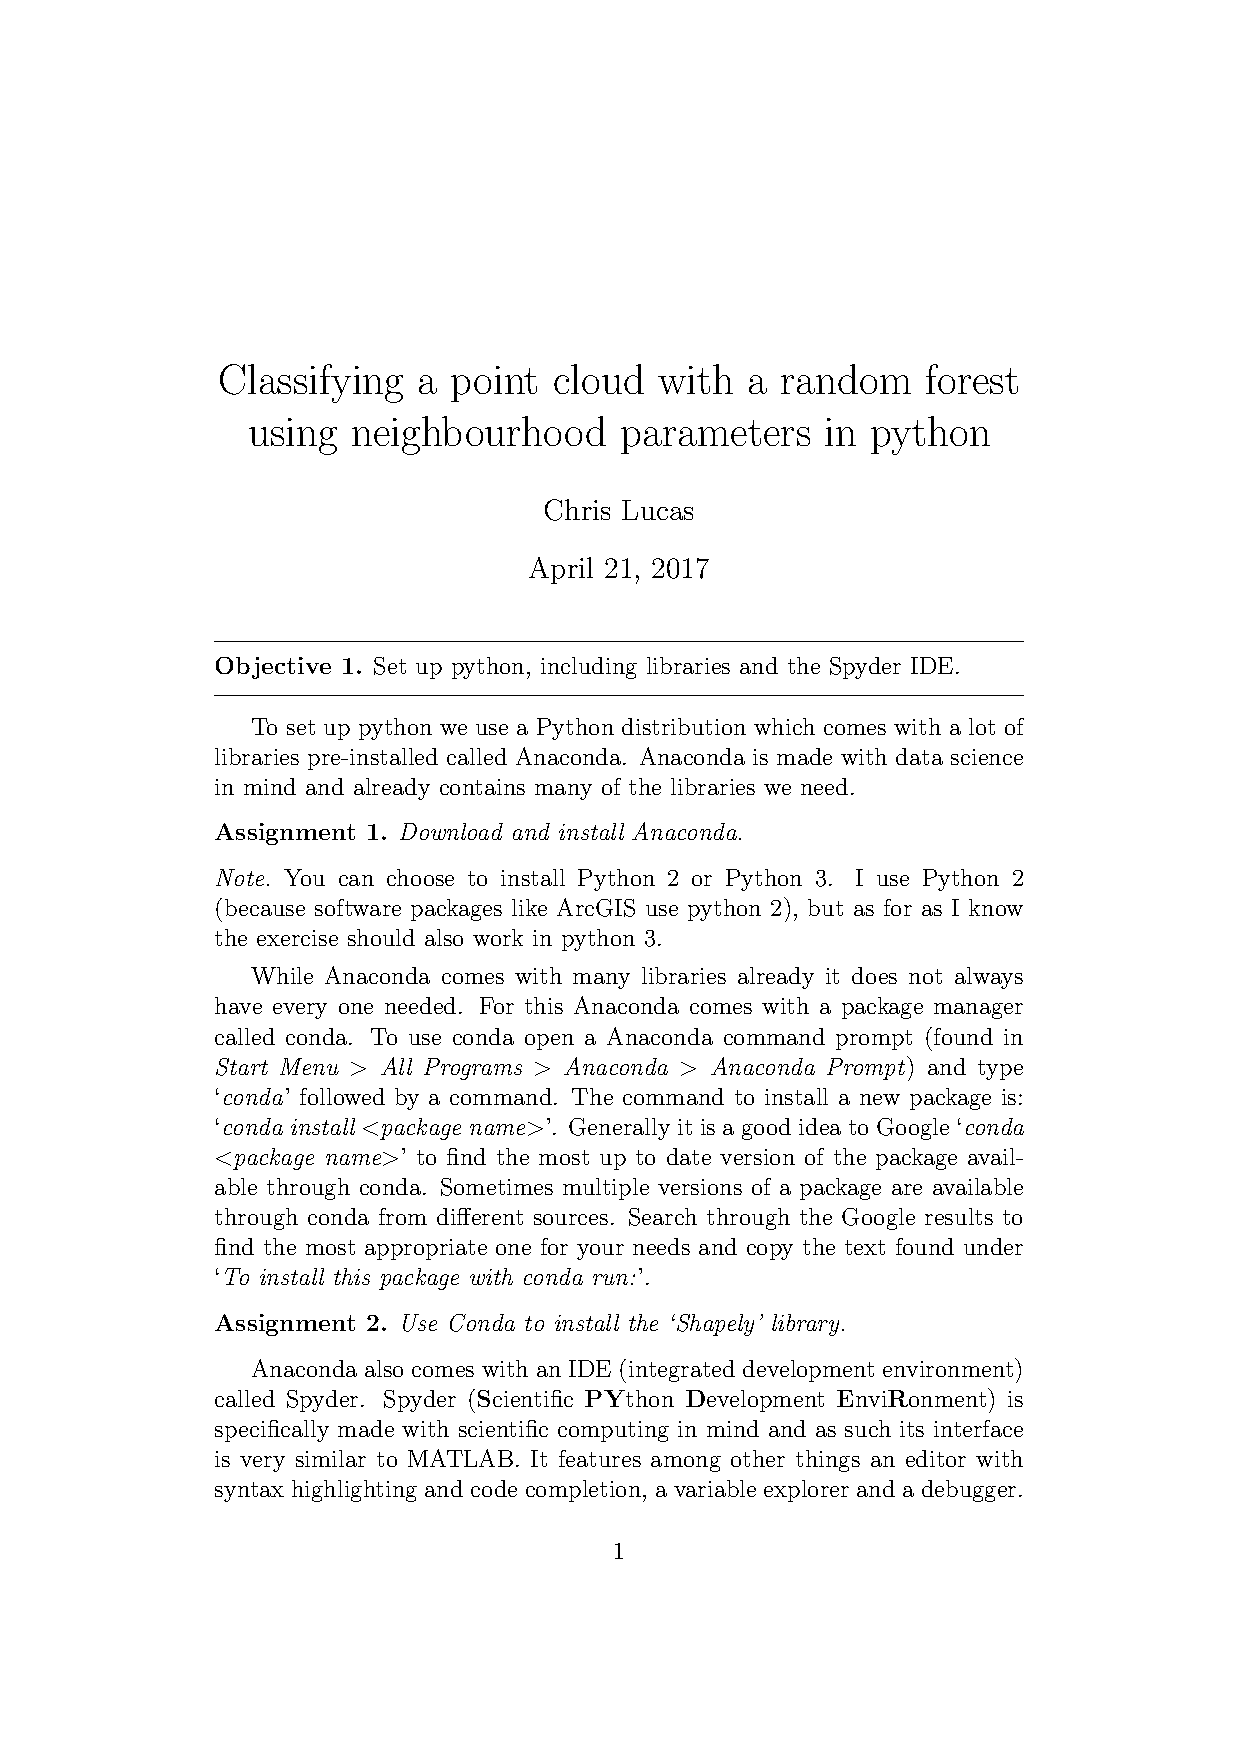
\includepdf[pages={-}]{./img/Assignment.pdf}